\documentclass[professionalfonts]{beamer}
\usepackage[utf8]{inputenc}
\usepackage[russian]{babel}
\usepackage{fancybox}
\usepackage{pdfpages}
\usepackage{listings}
\usepackage{tikz-cd}
\usetheme{Pittsburgh}
\usecolortheme{owl}
\title{Состязательный поиск}
\begin{document}
\newcommand{\tictactoe}[9]{
	\begin{tabular}{c|c|c}
		#1 & #2 & #3 \\ \hline
		#4 & #5 & #6 \\ \hline
		#7 & #8 & #9
	\end{tabular}
	}

\newcommand{\cg}[1]{{\color{green}#1}}
\newcommand{\cy}[1]{{\color{yellow}#1}}

\frame{\titlepage}
\begin{frame}\fontsize{55}{55}\selectfont
	\centering
	\tictactoe{\;}{O}{X}
		{O}{X}{X}
		{O}{O}{X}
\end{frame}

\begin{frame}
	\fontsize{55}{55}\selectfont
	\centering
	\tictactoe{\;}{O}{\cg{X}}
		{O}{X}{\cg{X}}
		{O}{O}{\cg{X}}
\end{frame}
\begin{frame}
	\centering
	\begin{tabular}{c c c}
	\tictactoe
		{\cg{O}}{ X} { X}
		{\cg{O}} { O }{\;}
		{\cg{O}} { X }{ X}
		&
		\tictactoe
		{X}{ O} { X} 
		{O}{ O} { X }
		{X} {X} {O}
		&
		\tictactoe
			{O}  {\;}   {\cg{X}}
			{\;} {\cg{X}} {O}
			{\cg{X}} {O} {X}
		 \\
		-1 & 0 & 1
	\end{tabular}

\end{frame}


\begin{frame}
	\frametitle{Минимакс}
	\begin{itemize}
		\item max(X) максимизирует счёт
		\item min(O) минимизирует счёт
	\end{itemize}
\end{frame}
\begin{frame}
	\frametitle{Игра}
	\begin{itemize}
		\item $S_0$ - начальное состояние
			\pause
		\item Игрок(s) вычисляет, кто следующий ходит в состоянии s
			\pause
		\item Действия(s) вычисляет допустимые шаги в состоянии s
			\pause
		\item Результат(s, a) вычисляет состояние после шага a из состояния s
			\pause
		\item Конец(s) проверяет, что состояние s конечное
			\pause
		\item Оценка(s) вычисляет числовое значение конечного состояния s
				
	\end{itemize}
\end{frame}

\begin{frame}
	\frametitle{Начальное состояние}
	\fontsize{55}{55}\selectfont
	\centering
	\begin{tabular}{c|c|c}
		\;\;& \;\; &\;\;  \\ \hline
		 &  & \\ \hline
		 &  &  
	\end{tabular}
\end{frame}
\begin{frame}
	\frametitle{Игрок(s)}
	
	\bigskip

	\onslide<2->{Игрок(} \onslide<1->{ \begin{tabular}{c|c|c}
		\;&\;&\;\\ \hline
		& & \\ \hline
		& &
	\end{tabular}} \onslide<2->{ ) = X} 

	\bigskip

	\onslide<4->{Игрок(}\onslide<3->{\begin{tabular}{c|c|c}
		\;&\;&\;\\ \hline
		&X & \\ \hline
		& &
	\end{tabular}} \onslide<4->{) = O }
\end{frame}

\begin{frame}
	\frametitle{Действия(s)}

	\bigskip
	\onslide<1->{Действия(\begin{tabular}{c|c|c}
		\;& X & O\\ \hline
		O &X & X\\ \hline
		X& &O
	\end{tabular} ) =} \onslide<2->{\{
		\tictactoe
			{\cy{o}}{\;}{\;}
			  {\;}{\;}{\;}
			  {\;}{\;}{\;} ,}
		\onslide<3->{  \tictactoe
			  {\;}{\;}{\;}
			  {\;}{\;}{\;}
			 {\cy{o}}{\;}{\;} }
	\onslide<2->{\}}
\end{frame}
\begin{frame}
	\frametitle{Результат(s, a)}

	\bigskip

	\onslide<1->{	Результат 
		(
		\begin{tabular}{c|c|c}
			\;& X & O\\ \hline
			O &X & X\\ \hline
			X& &O
		\end{tabular} \;,\; 
		\begin{tabular}{c|c|c}
			{\color{yellow} o}&\;&\;\\ \hline
			& & \\ \hline
			& &
		\end{tabular} 
		) =}
		\onslide<2->{	\begin{tabular}{c|c|c}
				O&X&O\\ \hline
				O&X &X \\ \hline
				X& &O
		\end{tabular} }
\end{frame}
\begin{frame}
	\frametitle{Конец(s)}

	\bigskip

	Конец( 
	\begin{tabular}{c|c|c}
		O&   & \\ \hline
		O& X & \\ \hline
		X& O & X
	\end{tabular} 
		) = false
\pause
	\bigskip

	Конец( 
		\begin{tabular}{c|c|c}
			O&  & X \\ \hline
			O& X & \\ \hline
			X& O & X
		\end{tabular} 
		) = true

\end{frame}
\begin{frame}
\frametitle{Оценка(s)}
	Оценка(
	\tictactoe
			{O}{}{X}
			{O}{X}{} 
			{X}{O}{X}
	) = 1

	\bigskip
	\pause
	Оценка(
	\tictactoe
			{O}{}{X}
			{X}{O}{}
			{O} {X}{O}
	) = -1
\end{frame}
\begin{frame}
	\frametitle{Конечное(s)=true}
	\centering
	\begin{tabular}{c}
	Знач:\\
		1
	\end{tabular} 
	\begin{tabular}{c|c|c}
	 O& X & O \\ \hline
	O& X & X \\ \hline
		X& X & O
\end{tabular}  
\end{frame}
\begin{frame}[fragile]\fontsize{6}{12}\selectfont

\begin{tikzcd}
		Plaer(s)=O	&\begin{tabular}{c}
		MinV:\\
		0
		\end{tabular} 	\tictactoe
				{\,} {X}  {O}
				{O} {X}  {X} 
				{X} {\,} {O}
	\arrow{ld}\arrow{rd}		 &  \\
	\begin{tabular}{c}
		MaxV:\\
		1
	\end{tabular} 
	\tictactoe
	{\cy{O}} {X} { O}
	{O} {X} { X}
	{X} {} { O}
	\arrow{d}		&			&
					\begin{tabular}{c}
						MaxV:\\
						0
					\end{tabular} 
						\tictactoe
						{} {X} {O}
						{O}{ X} { X}
						 {X} {\cy{O}}{O}\arrow{d} 	\\
\begin{tabular}{c}
	Val:\\
		1
	\end{tabular} 
	\tictactoe
	{\cy{O}}{X}{O}
	{O}   {X} { X}
	{X} {\cy{X}} {O}
	&			&
					\begin{tabular}{c}
						Val:\\
						0
					\end{tabular} 
					\tictactoe
						{\cy{X}}{X}{ O}
						  {O}  {X}  {X}
						 {X} {\cy{O}}{O}
\end{tikzcd}
\end{frame}
{
\setbeamercolor{background canvas}{bg=}
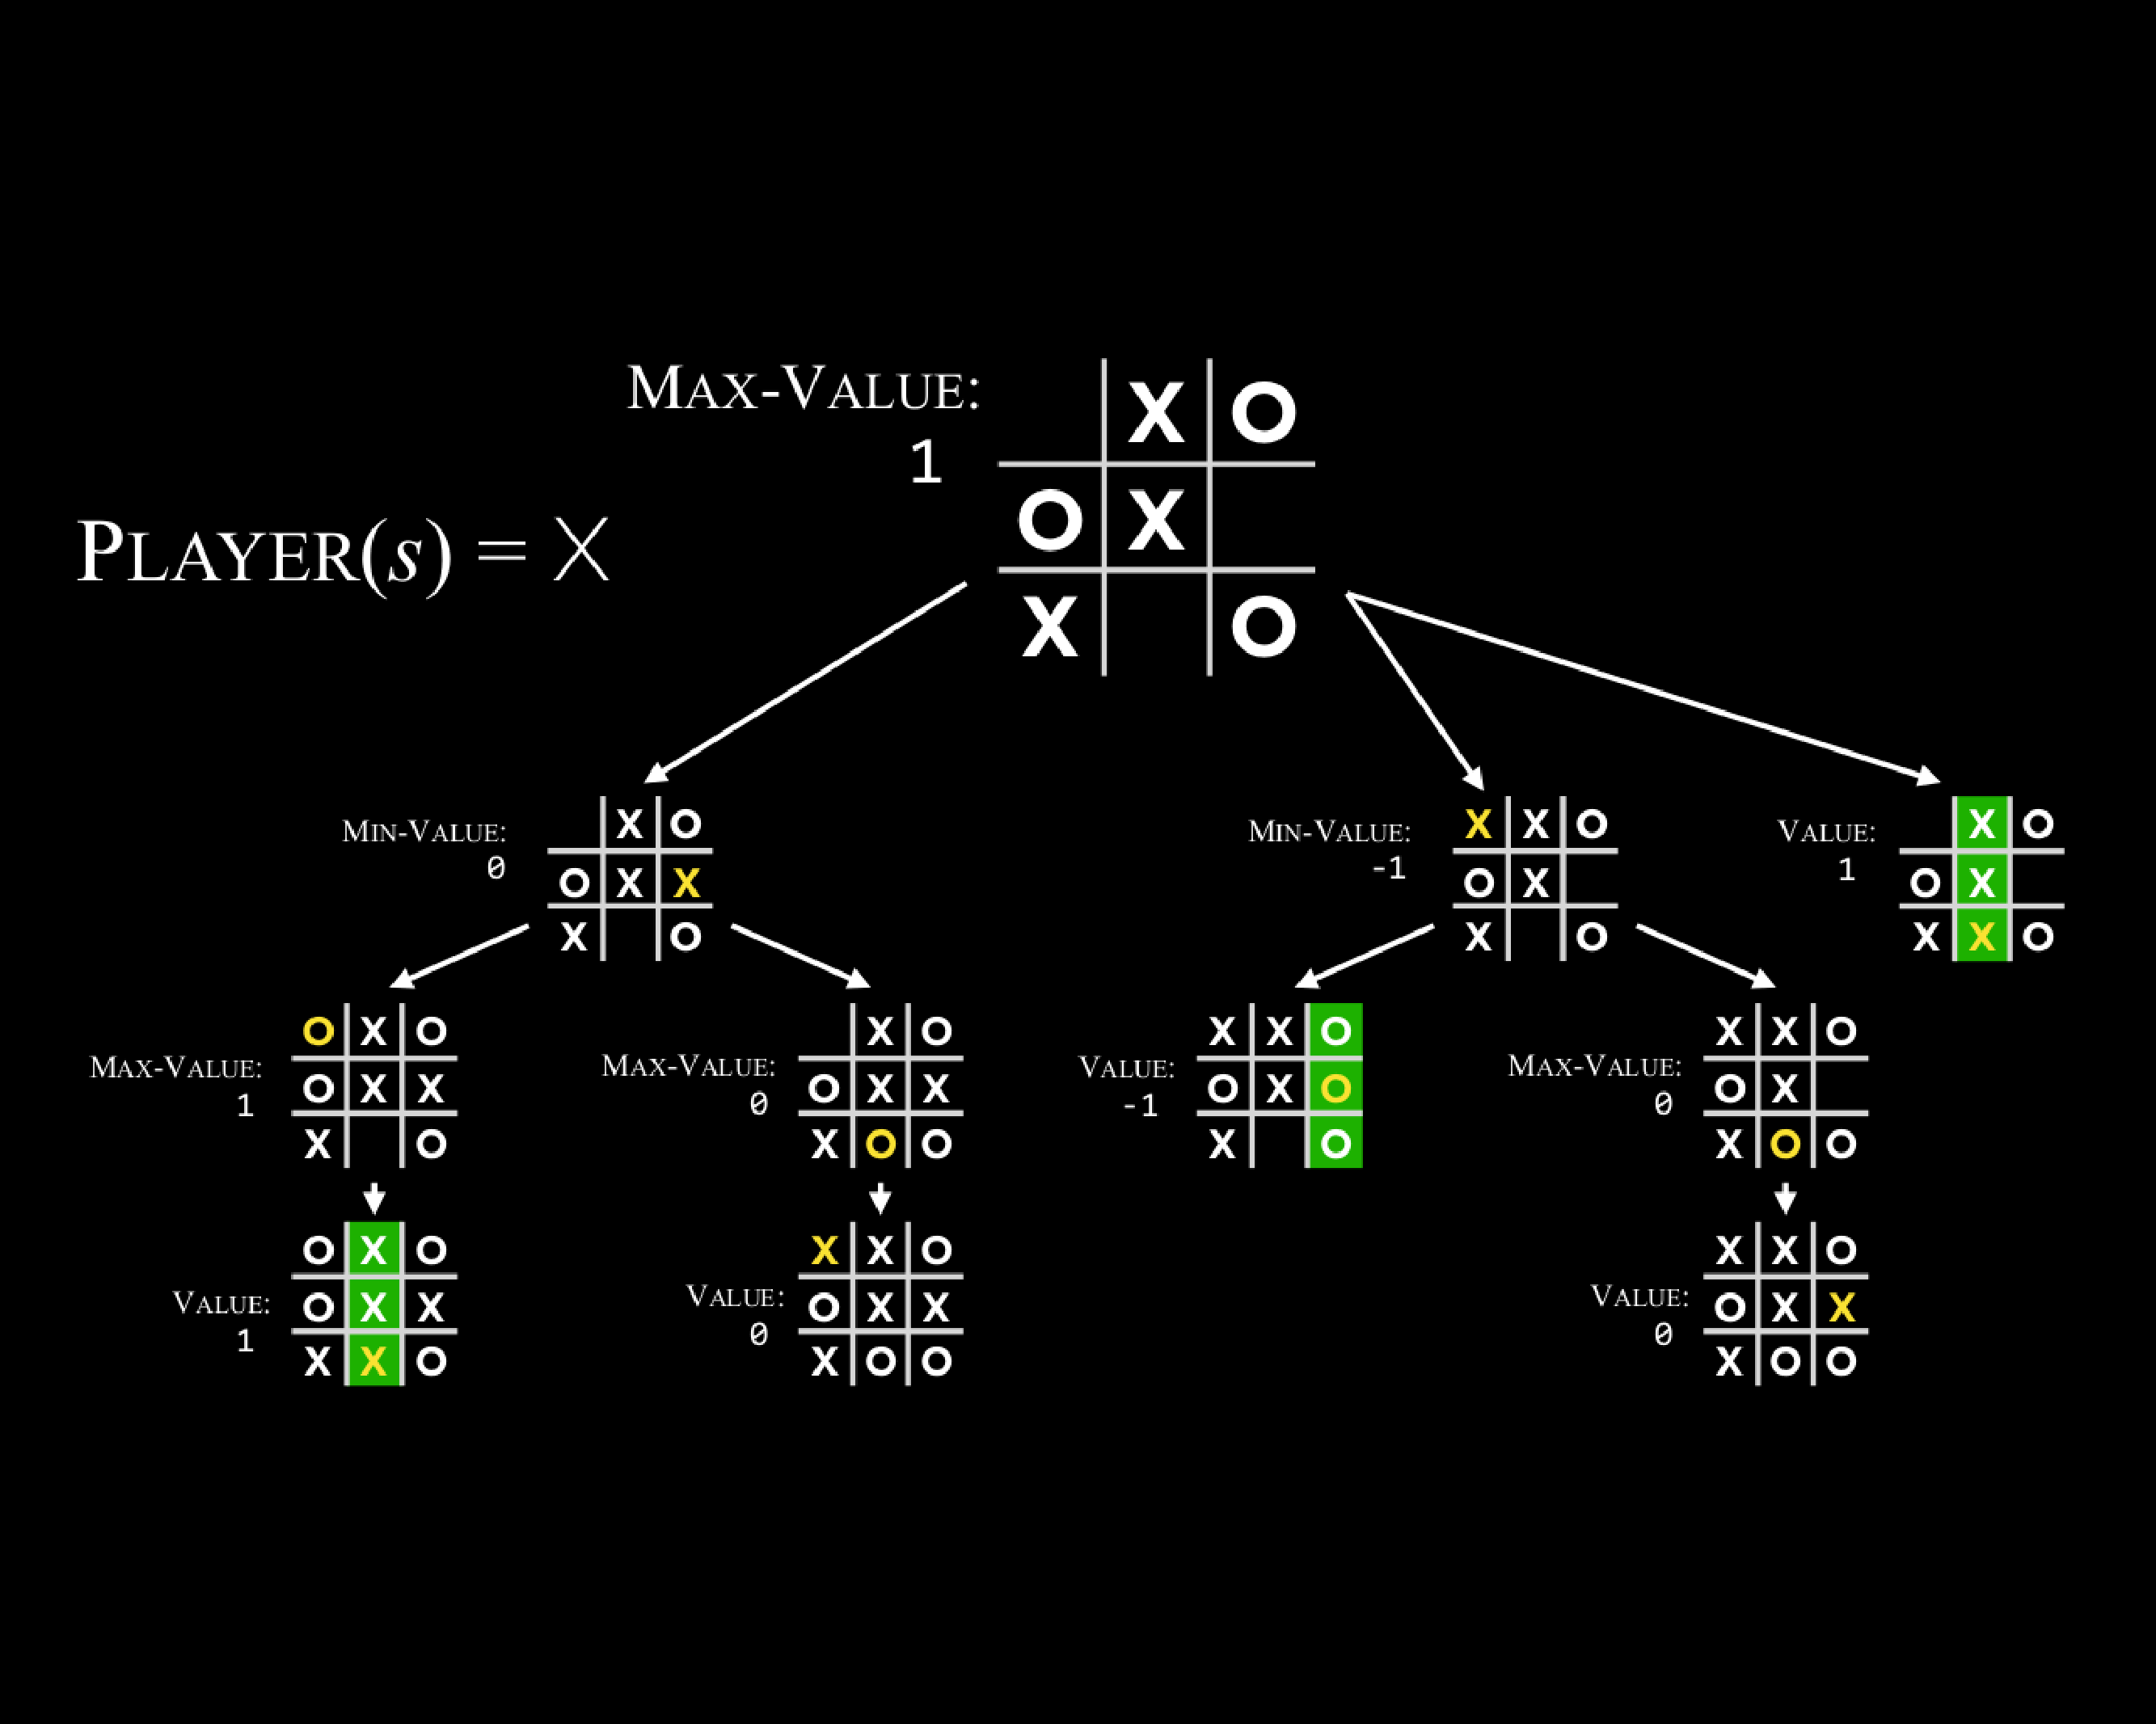
\includepdf{test13.pdf}
}
{
\setbeamercolor{background canvas}{bg=}
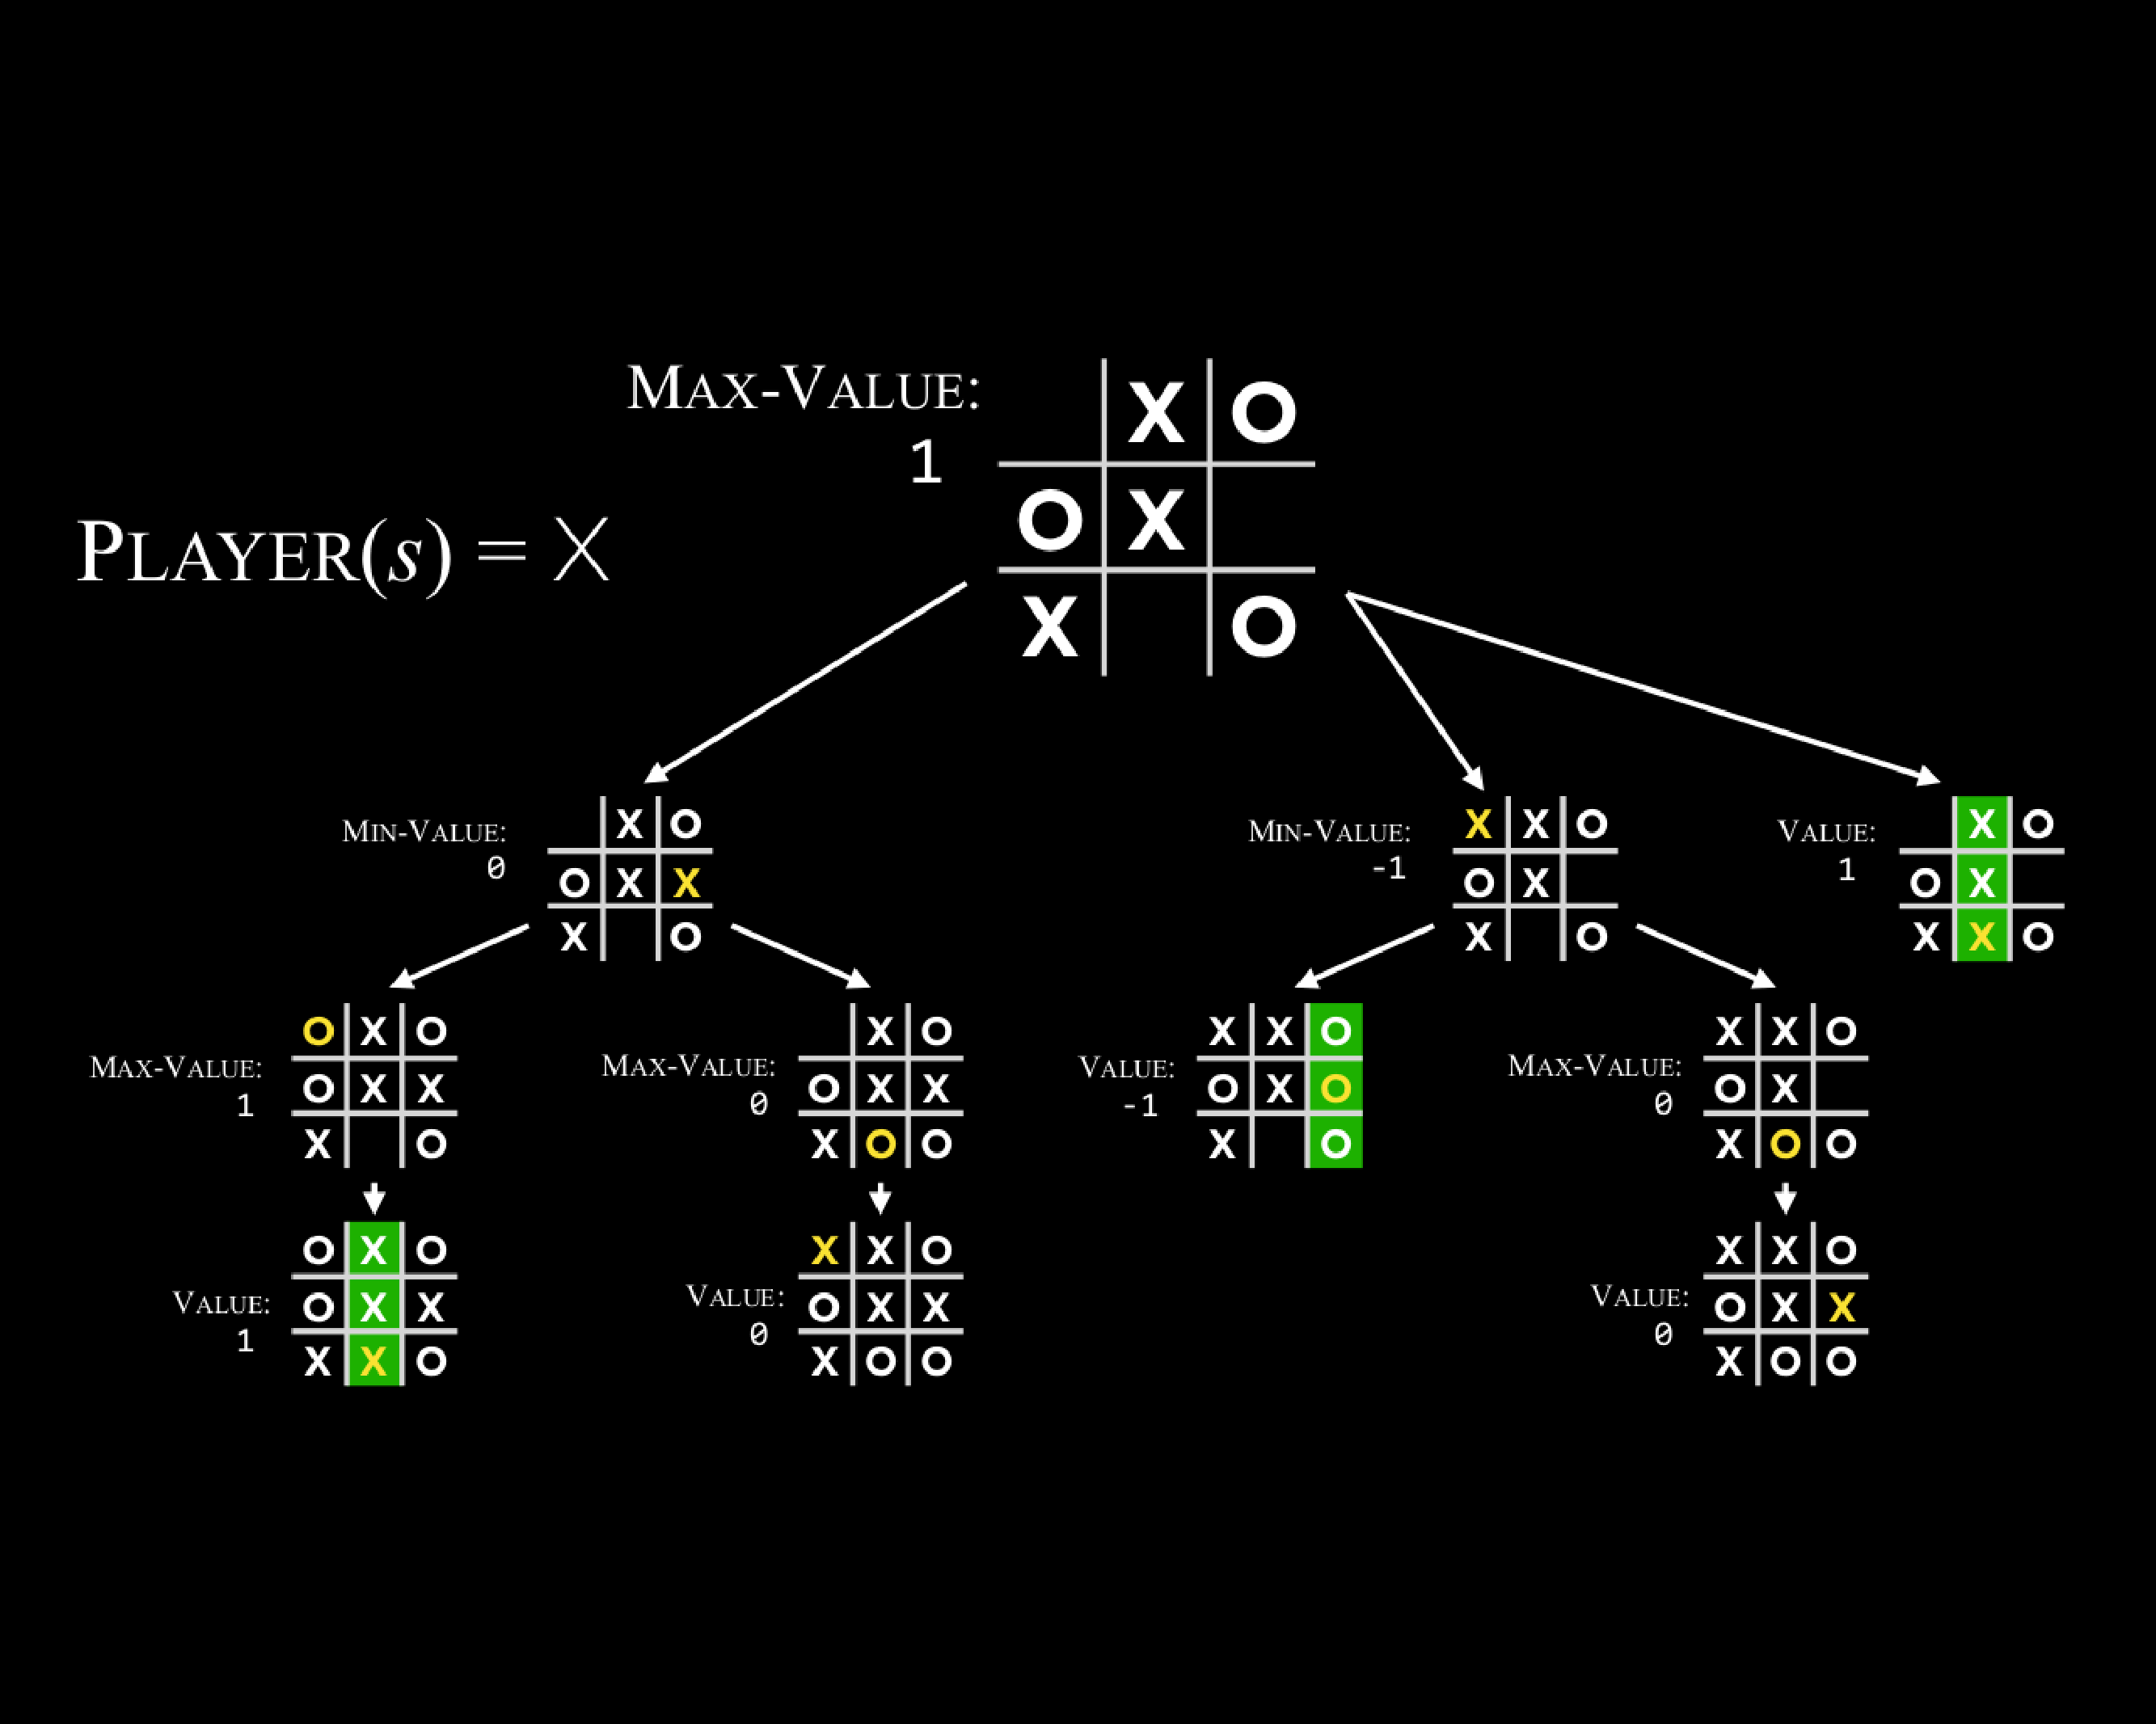
\includepdf{test14.pdf}
}
{
\setbeamercolor{background canvas}{bg=}
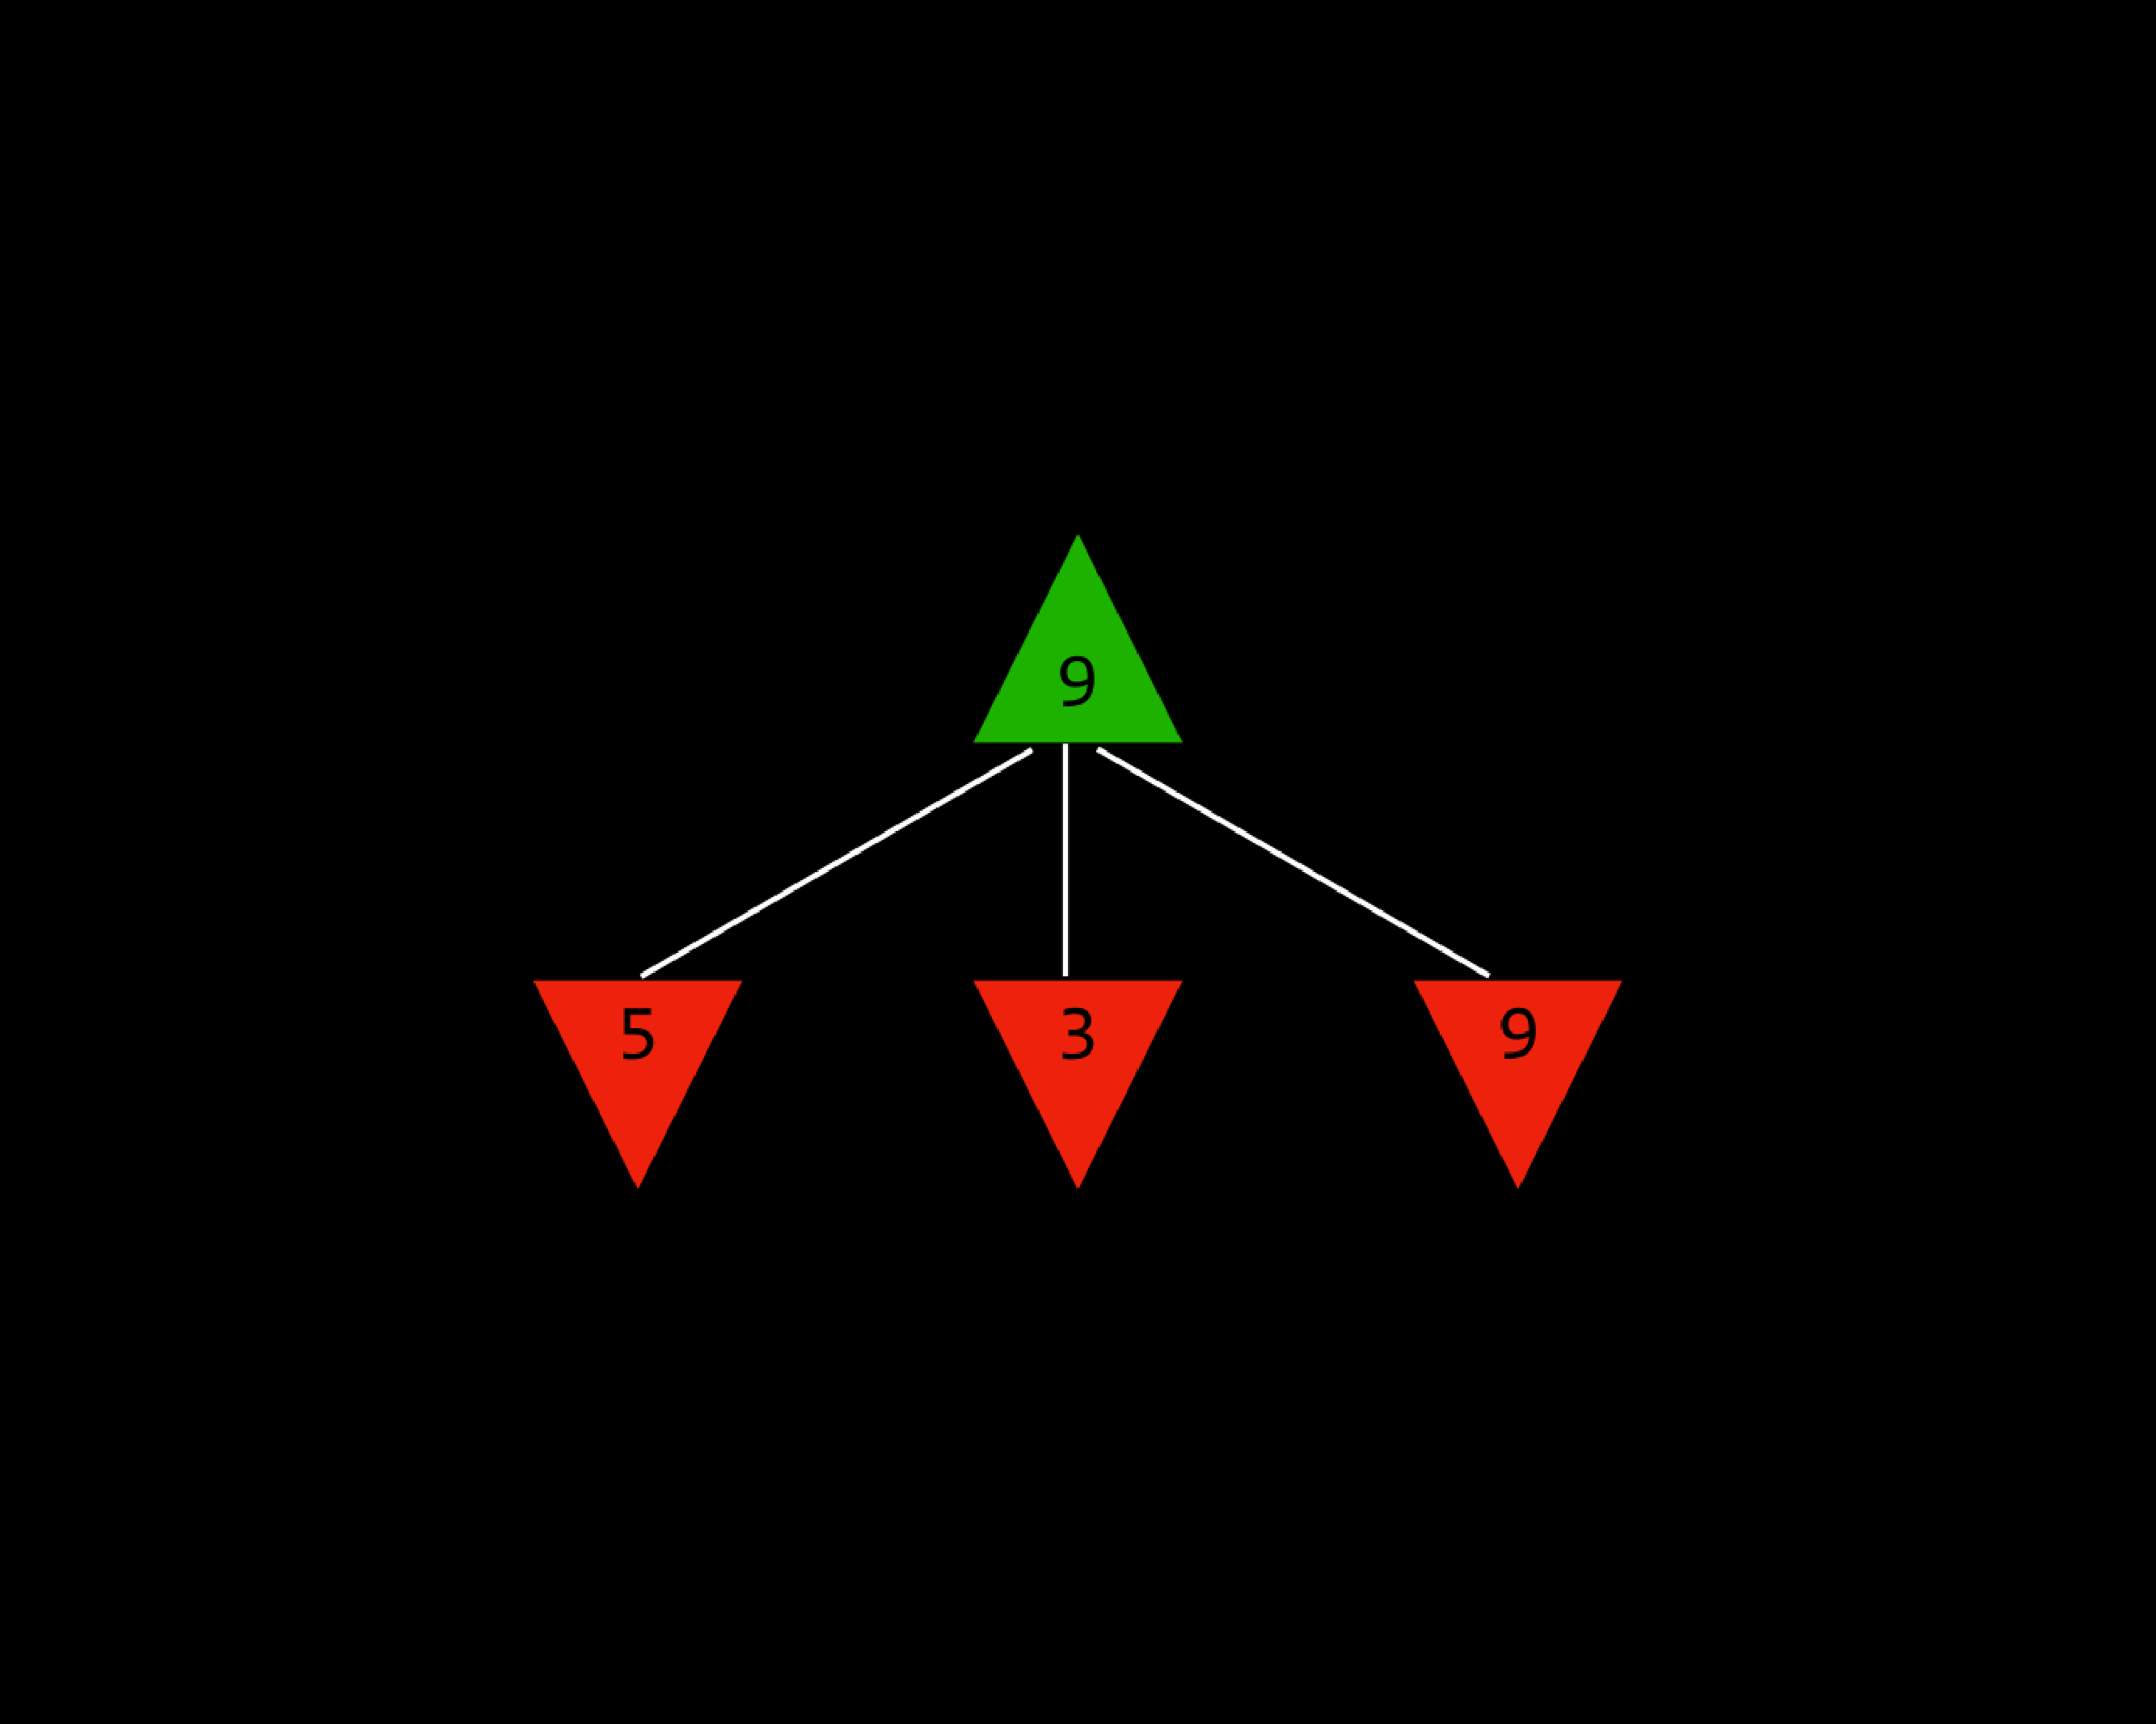
\includepdf{test15.pdf}
}
{
\setbeamercolor{background canvas}{bg=}
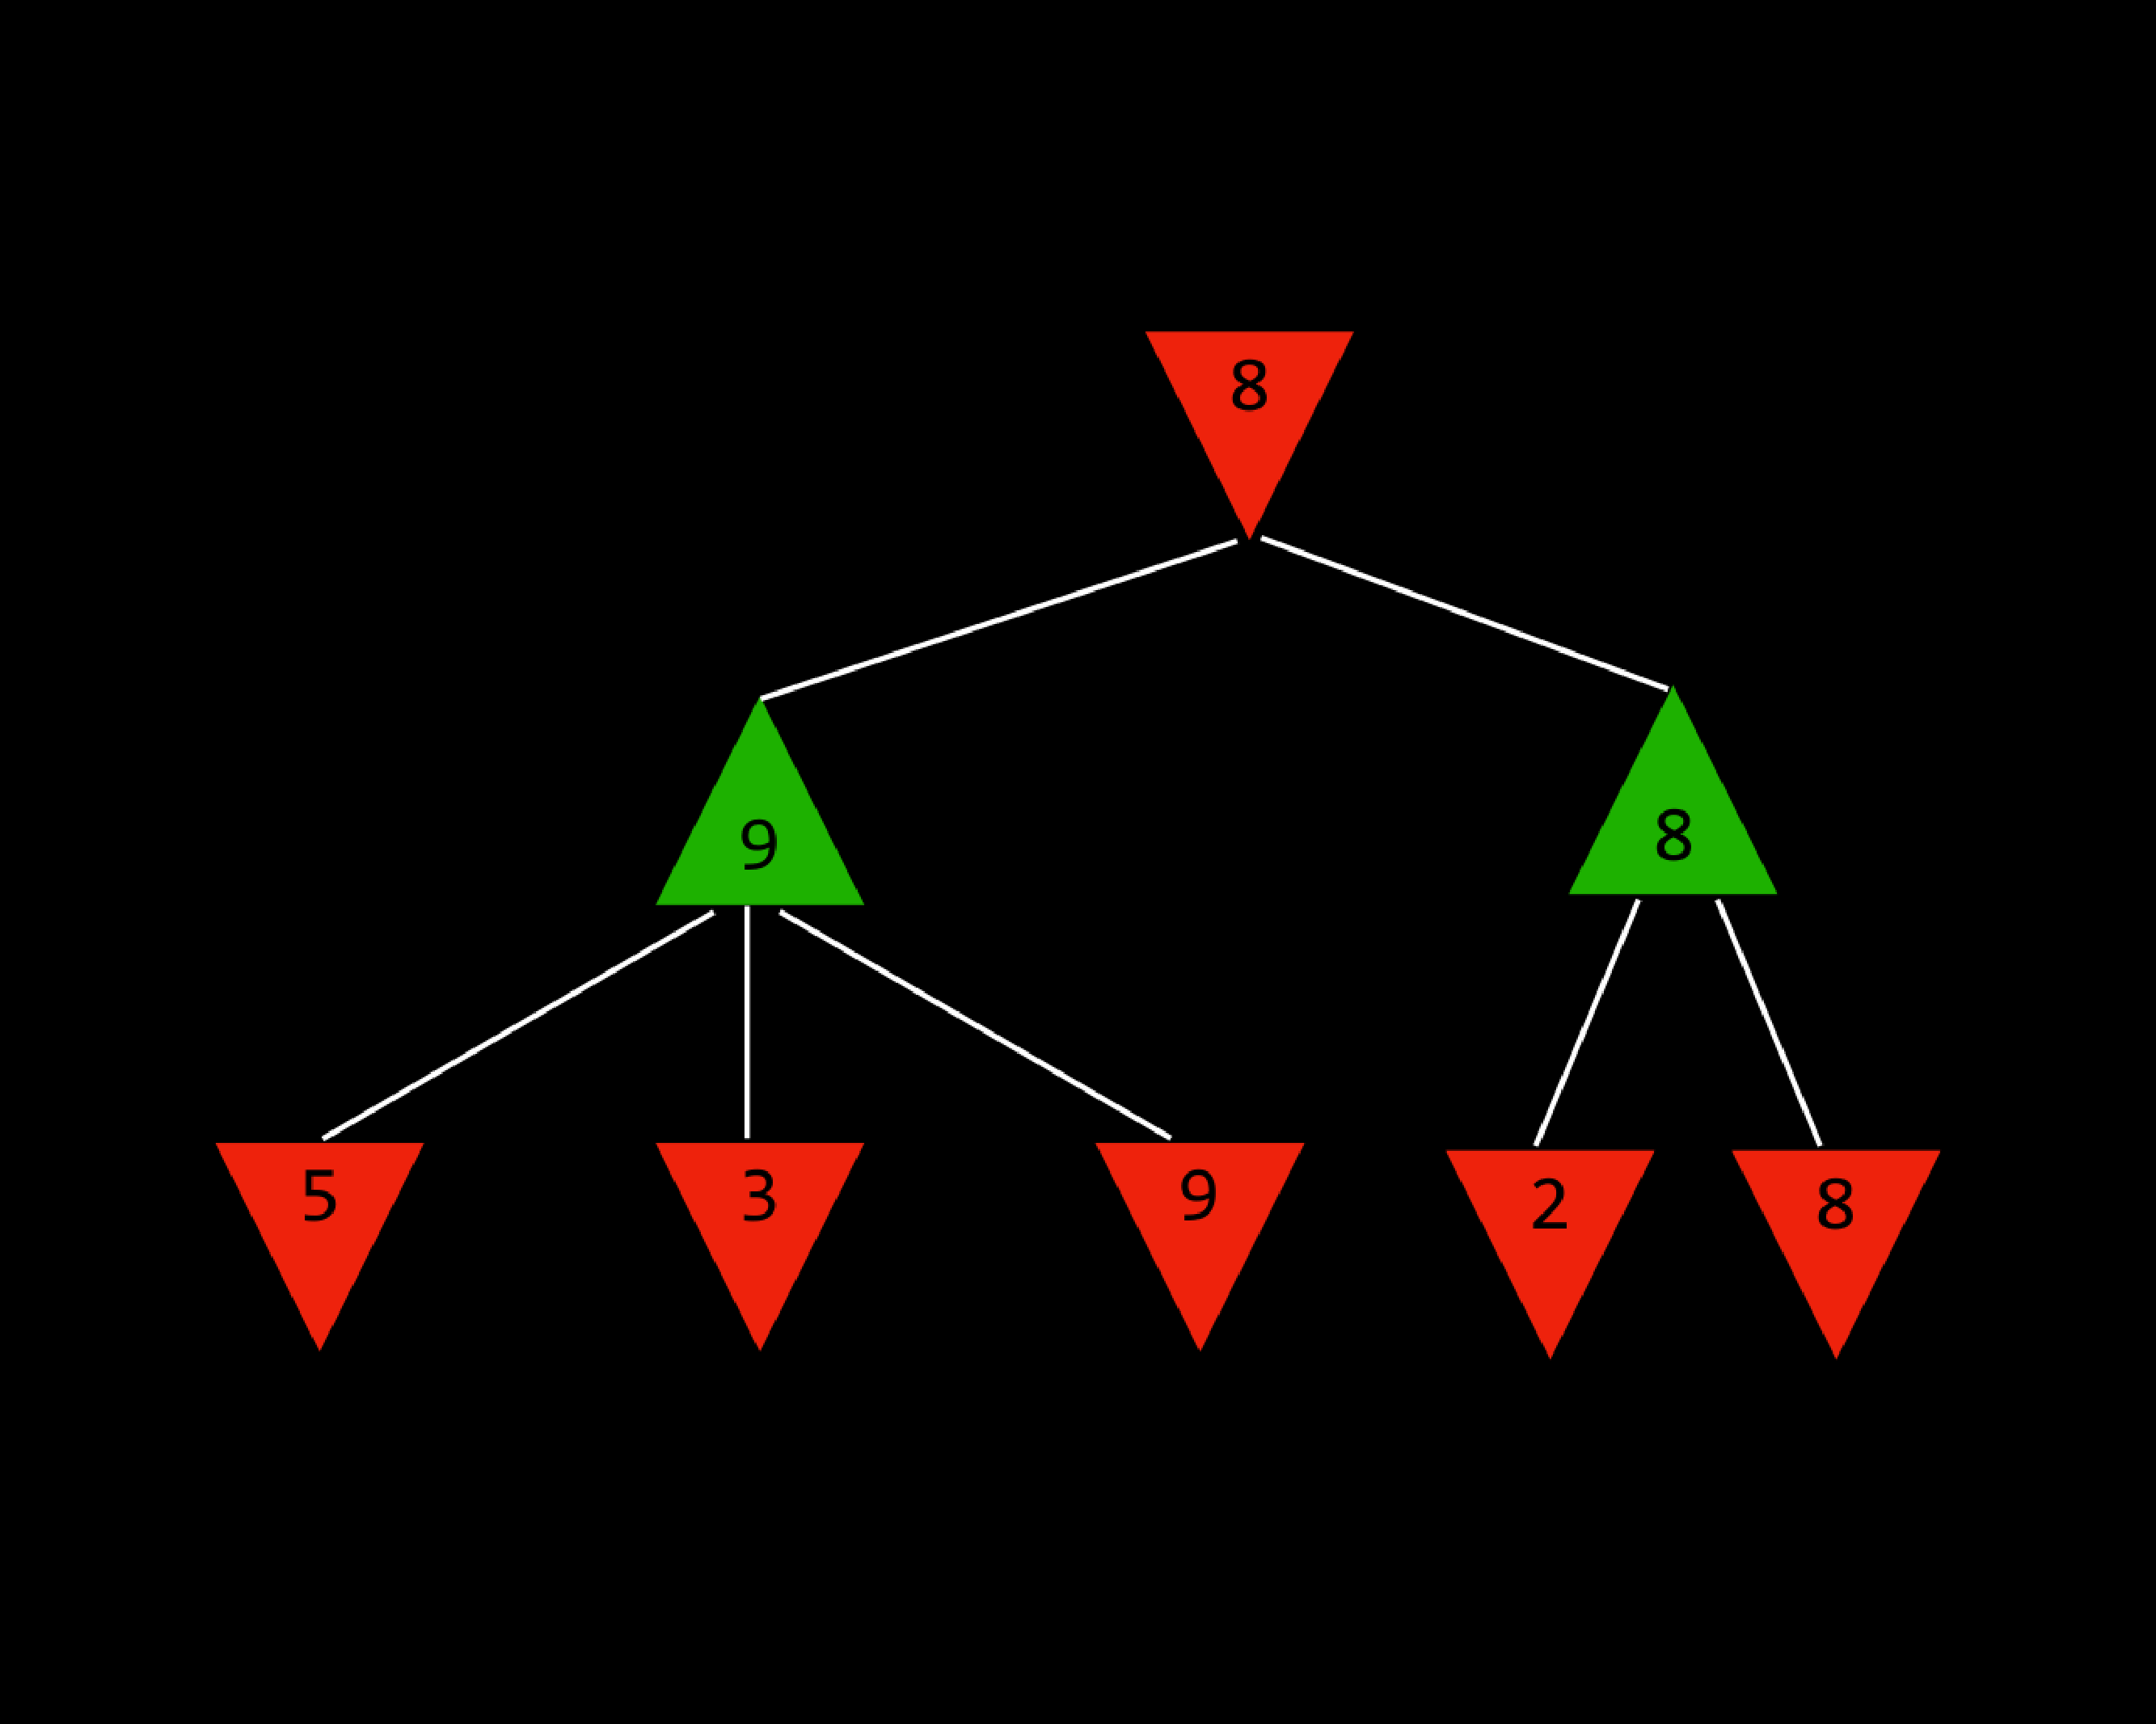
\includepdf{test16.pdf}
}

\begin{frame}
	\frametitle{Минимакс}
		\begin{itemize}
				\item Дано состояние s:
			\begin{itemize}
				\item МАКС выбирает действие a из Действия(s), для которого  функция Мин-значение(Результат(s, a)) принимает максимальное значение 
				\item МИН выбирает действие a из Действия(s), для которого функция Макс-значение(Результат(s, a)) принимает минимальное значение
		\end{itemize}
		\end{itemize}
\end{frame}

\begin{frame}
	\frametitle{Минимакс}
	функция Макс-значение(состояние):

	\hspace{20pt}
		если Конец(состояние):

		\hspace{40pt}	возвращаем Оценка(состояние)

		\hspace{20pt}$v = -\infty$

		\hspace{20pt}для действия в Действия(состояние):

		\hspace{40pt}	$v$ = Макс($v$, Мин-значение(Результат(состояние, действие)))

		\hspace{20pt}
		вернуть $v$
\end{frame}
\begin{frame}
	\frametitle{Минимакс}
	функция Мин-значение(состояние):

	\hspace{20pt}
		если Конец(состояние):

		\hspace{40pt}	возвращаем Оценка(состояние)

		\hspace{20pt}$v = \infty$

		\hspace{20pt}для действия в Действия(состояние):

		\hspace{40pt}	$v$ = Мин($v$, Макс-значение(Результат(состояние, действие)))

		\hspace{20pt}
		вернуть $v$
\end{frame}

\end{document}
